\documentclass{report}
\usepackage[utf8]{inputenc}
\usepackage{enumitem}
\title{Assignment 9 (GATE, EC2017,45)}
\author{Suhani Kalra }
\date{16 December 2020}

\usepackage{circuitikz}
\usepackage{array}

\begin{document}
\maketitle
\section{QUESTION}
\begin{figure}[htp]
        \centering
        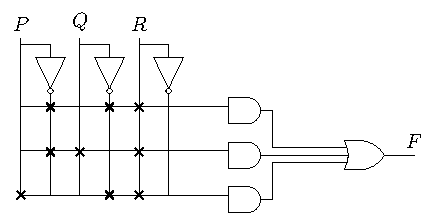
\includegraphics[width=17cm]{image.pdf}
        \caption{GATE, EC2017,45}
        \label{fig:ok}
\end{figure}
\huge
A programmable logic array (PLA) is shown in the figure.The Boolean function F implemented is

 \begin{enumerate}
 \item P'Q'R+PQ'R+P'QR
\item ( P'+Q'+R)(P'+Q+R)(P+Q'+R')
\item P'QR+PQ'R+PQR
\item ( P+Q'+R)(P'+Q+R)(P+Q'+R')
  \end{enumerate}





\newpage
\section{Programmable Logic Array}
 It is a kind of programmable logic device used to implement combinational logic circuits.It has a Programmable AND array as well as fixed OR array.The structure of PLA allows its inputs (and their complement) to be AND’ed together in the AND plane which will correspond to the product term of its inputs. Also, each output of the OR plane can be configured to give the logical sum of any outputs of the AND plane. This structure allows the implementation of logic functions in the sum-of-products form.In PLA, all the minterms are not realized but only required minterms are implemented.Its applications are:
 \begin{enumerate}
 \item To provide control over datapath.

\item Used as a counter.

\item Used as decoders.
\end{enumerate}

\newpage
\section{SOLUTION}
For the question 45 of GATE EC 2017 exam(Figure 1, Section 0.1),
\newline
    we had to deduce the expression for the final Output F from the PLA, given in the Figure 1 (section0.1) for this, we can say that, Figure 1 could be reduced to the following equation
\begin{equation}
   \textcolor{blue}{F = P'Q'R+PQ'R+P'QR}
\end{equation}
 The following report aims at providing a detailed derivation of the equation1 using,Truth Table and Logical Circuit Diagram.

\newpage
\section{CIRCUIT DIAGRAM}

The given question (figure 1, section 0.1 ) can also be represented by the following circuit diagram. This circuit diagram helps us to deduce the above mentioned equation1 (section0.2).
\begin{figure}[h]\centering
\begin{circuitikz}

\ctikzset{tripoles/american and port/height=1.1, number inputs=3 };
\ctikzset{tripoles/american or port/height=1};
\draw

    (2,0.7)node[american or port, number inputs=3, anchor=in 1](OR1) {} 
    (-1.4,-1) node[american and port, number inputs=3, anchor=in 1](a){PQ'R}
    (-1.4,0.7) node[american and port, number inputs=3, anchor=in 1](C){P'Q'R}
    (-1.4,2.5) node[american and port, number inputs=3, anchor=in 1](b){P'QR}

    (C.in 1) node[anchor=east] {P}
    (C.in 2) node[anchor=east] {Q}
    (C.in 3) node[anchor=east] {R}
    (b.in 1) node[anchor=east] {P}
    (b.in 2) node[anchor=east] {Q}
    (b.in 3) node[anchor=east] {R}
    (a.in 1) node[anchor=east] {P}
    (a.in 2) node[anchor=east] {Q}
    (a.in 3) node[anchor=east] {R}
    (OR1.out) node[anchor=west] {$F$}
    (a.out)--(OR1.in 3)
    (b.out)--(OR1.in 1)
    (C.out)--(OR1.in 2);
    \node at (b.bin 1) [ocirc, left]{} ;
    \node at (C.bin 2) [ocirc, left]{} ;
    \node at (C.bin 1) [ocirc, left]{} ;
    \node at (a.bin 2) [ocirc, left]{} ;
    \end{circuitikz}
    \end{figure}

\newpage
\section{TRUTH TABLE}

The given question (figure 1, section 0.1 ) can also be represented by the aforementioned Truth Table. This Truth table helps us to deduce the above mentioned equation1 (section0.3).
\begin{table}[]\centering
  \begin{tabular}{|l|l|l|l|}
  \hline
        P & Q & R & F  \\ \hline
        0 & 0 & 0     & 0         \\
        0 & 0 & 1     & 1         \\
        0 & 1 & 0     & 0         \\ 
        0 & 1 & 1     & 1         \\
        1 & 0 & 0     & 0         \\
        1 & 0 & 1     & 1         \\
        1 & 1 & 0     & 0         \\
        1 & 1 & 1     & 0         \\ \hline

\end{tabular}
\end{table}


\end{document}
